% Niveau :      PCSI *
% Discipline :  Chimie Orga
% Mots clés :   Stéréochimie

\begin{exercise}{Spectre RMN du [18]annulène}{3}{PCSI}
{Chimie organique I,Spectroscopie,RMN}{bermu}

\begin{questions}
\questioncours RMN du proton $^{1}$H. Réalisation d'un spectre, principe de fonctionnement. Déplacement chimique $\delta$ : influence de l'environnement chimique et du solvant.

\question Commentez les spectres RMN du [18]annulène :
\end{questions}

\noindent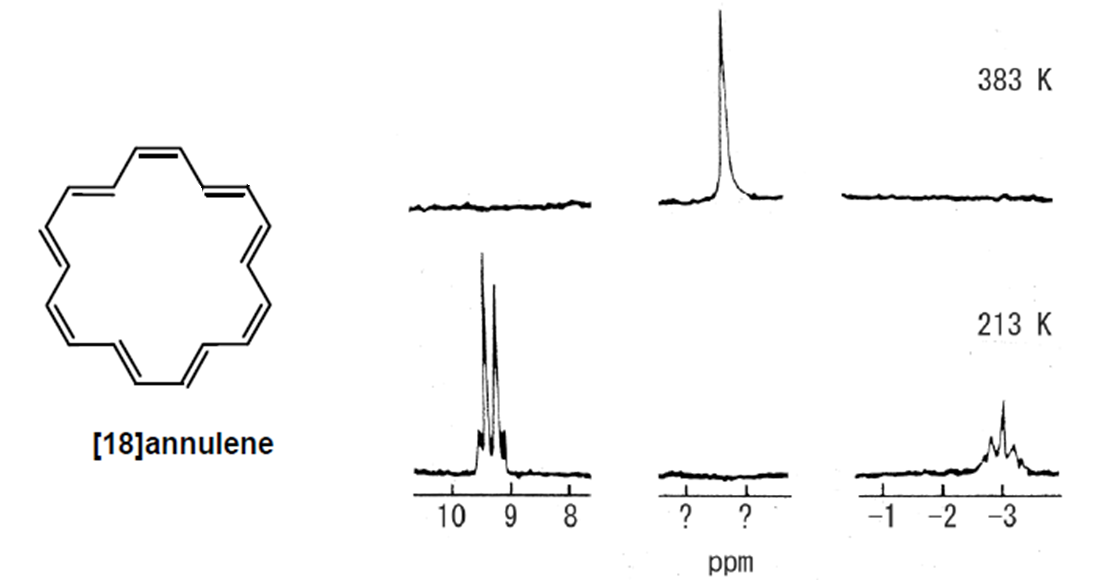
\includegraphics[width=\linewidth]{chimiePC/orga/annulene.png}

\end{exercise}